\documentclass[12pt,a4paper]{article}

\usepackage{german}      % Deutsche TeX-Eigenheiten
%\usepackage{isolatin1}   % Eingabekodierung mit Umlauten...
\usepackage{hyperref}
\usepackage{makeidx}
\makeindex            % damit eine Indexdatei angelegt wird

\usepackage{graphicx}

\usepackage{amsmath}  % allgemeine Mathe-Erweiterungen
\usepackage{amssymb}  % Symbole und Schriftarten
\usepackage{amsthm}   % erweiterte Theorem-Umgebungen

\usepackage{mathrsfs}  % gibt den Befehl "\mathscr{}" f�r sch�ne

\begin{document}

\section{Tutorial 1 - Taylor}
\subsection{Zusammenfassung}
\underline{Zweck:}\\
- beliebige Funktion als Polynom mit Fehler darstellen = Approximieren\\
- Wenn f im Intervall I[a,b] (n+1)-mal stetig differenzierbar\\
dann gilt für alle x Element I die Taylorsche Formel:\\
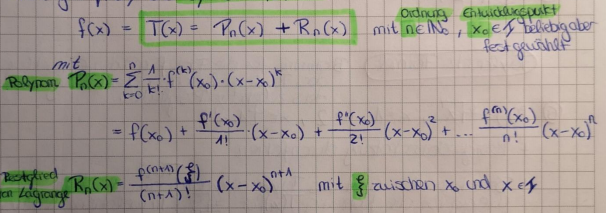
\includegraphics[width=1\textwidth]{Bilder/1.png}\\
\href{http://www.mathematik.net/reihen-taylor-polynome/tp2s41.htm}{Taylorpolynome}.
\subsubsection{Fehlerabschätzung des Restglieds}
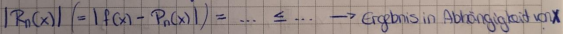
\includegraphics[width=0.8\textwidth]{Bilder/2.png}\\
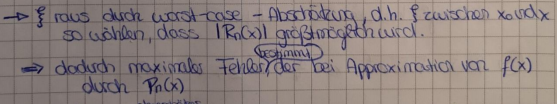
\includegraphics[width=0.8\textwidth]{Bilder/3.png}\\
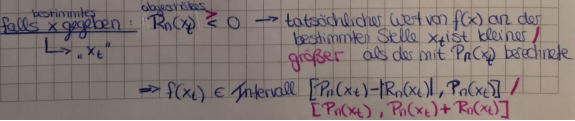
\includegraphics[width=0.8\textwidth]{Bilder/4.png}\\
\end{document} 